\section{Эксперементальная часть.}

В качестве диода используется электронная лампа 2Ц2С с цилиндрическим анодом и соосным с ним катодом ($r_k \leq r_a$). Диод помещен в соленоид ,ось симметрии которого совпадает с осью симметрии электродов лампы. При пропускании через соленоид постоянного тока и подаче на анод положительного потенциала в диоде реализуются скрещенные электрические и магнитные поля, характерные для магнетрона. 

Для экспериментального определения зависимости анодного тока диода от тока соленоида служит установка, схема которой показана на рис. \ref{fig:image3}. Напряжение на электроды вакуумного диода подается от специального источника питания УИП. Накал лампы питается переменным напряжениемем $~ 2,15$ В. Разность потенциалов между анодом и катодом регулируется соответствующей ручкой источника питания. Измеряется анодное напряжение вольтметром $V_a$, находящимся на панели источника питания. Анодный ток измеряется миллиамперметром, смонтированным вместе с соленоидом на специальной плате. Соленоид $C$ питается от сети постоянного напряжения 110 В. Величина тока в соленоиде регулируется с помощью реостата $R_c$ и измеряется амперметром $I_c$. Соленоид допускает ток до 1 А.

\begin{figure}[!h]
    \centering
    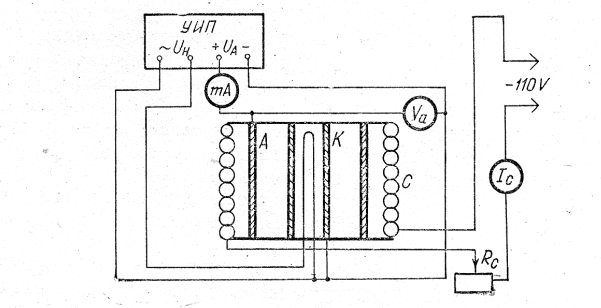
\includegraphics[width = 0.5\textwidth]{image/image3.png}
    \caption{Рис. 3}
    \label{fig:image3}
\end{figure}

Для экспериментальной установки, используемой в данной работе, имеют место следующие значения параметров:

$n_0 = 23400 \frac{1}{\text{м}}$ "--- число витков соленоида на единицу длины;

$l = 0.23$ м "--- длина соленоида;

$d = 0.1$ м "--- средний диаметр витков соленоида;

$r_a = 9.6 \cdot 10^{-3}$ м "--- радиус анода вакуумного диода.

Разбирать установку или производить какие"=либо изменения в ее схеме запрещается. На панели источника питания можно пользоваться лишь ручкой регулировки напряжения и тумблером <<сеть>>. Остальные ручки управления заблокированы и изменять их положение нельзя.

Лабораторную работу необходимо выполнять в следующем порядке:
\begin{enumerate}
    \item{ Включить в сеть переменного напряжения 220 В источник питания и поставить тумблер <<сеть>> в положение <<вкл>>. Через 1--2 минуты установить анодное напряжение $V_a = 150$ В. Подождать 2--3 минуты, необходимые для прогрева лампы. }
    \item{ Включить в сеть <<110 В>> с помощью специальной вилки питание соленоида. Изменяя величину тока $I_c$ в соленоиде с помощью реостата $R_c$, найти зависимость анодного тока от тока соленоида. Наиболее детальные измерения следует проводить на участке спада величины $l_a$. }
    \item{ Аналогичные измерения провести при анодных напряжениях $V_a = 200$ В и $V_a = 250$ В. Результаты измерений оформить в виде таблицы. }
    \item{ По экспериментальным данным для каждого значения анодного напряжения построить на <<миллиметровке>> зависимость $l_a = f(l_e)$. По графикам определить, как показано на рис. \ref{fig:image1}, величину критического тока в соленоиде $І_{ck}$. }
    \item{ По формуле (\ref{eq:formula4}) для каждого анодного напряжения рассчитать величины критической магнитной индукции $B_k$. }
    \item{ Вычислить для каждого анодного напряжения по формуле (\ref{eq:formula2}) величину удельного заряда электрона. Данные всех расчетов оформить в виде таблицы. Найти среднее значение удельного заряда электрона и сравнить его с табличным значением. }
\end{enumerate}



\begin{table}[!h]
    \centering
    \begin{tabular}{|c|c|c|c|c|c|}
         \hline
         \makecell{Замер 1\\($160B$)\\лампа} &
         \makecell{Замер 1\\($200B$)\\солиноид}&
         \makecell{Замер 2\\($200B$)\\лампа} &
         \makecell{Замер 2\\($200B$)\\солиноид}&
         \makecell{Замер 3\\($220B$)\\лампа} &
         \makecell{Замер 3\\($220B$)\\солиноид}\\
         \hline
         $30$& $0$& $40.5$& $0$& $48.5$& $0$\\
         \hline
         $29$& $0.29$& $40.5$& $0.2$& $48$& $0.25$\\
         \hline
         $23$& $0.34$& $40.5$& $0.23$& $47.5$& $0.32$\\
         \hline
         $21$& $0.35$& $40.25$& $0.25$& $46.5$& $0.36$\\
         \hline
         $18.5$& $0.37$& $40$& $0.29$& $39$& $0.39$\\
         \hline
         $17$& $0.38$& $39$& $0.34$& $32.5$& $0.42$\\
         \hline
         
    \end{tabular}
    \caption{Измерения}
    \label{tab:my_label1}
\end{table}
















